\documentclass[10pt,twocolumn,letterpaper]{article}

\usepackage{cvpr}
\usepackage{times}
\usepackage{epsfig}
\usepackage{graphicx}
\usepackage{amsmath}
\usepackage{amssymb}
\usepackage{subfigure}

% Include other packages here, before hyperref.

% If you comment hyperref and then uncomment it, you should delete
% egpaper.aux before re-running latex.  (Or just hit 'q' on the first latex
% run, let it finish, and you should be clear).
\usepackage[breaklinks=true,bookmarks=false]{hyperref}

\cvprfinalcopy % *** Uncomment this line for the final submission

\def\cvprPaperID{****} % *** Enter the CVPR Paper ID here
\def\httilde{\mbox{\tt\raisebox{-.5ex}{\symbol{126}}}}

% Pages are numbered in submission mode, and unnumbered in camera-ready
%\ifcvprfinal\pagestyle{empty}\fi
\setcounter{page}{1}
\begin{document}

%%%%%%%%% TITLE
\title{Praktikum: Virtual Neurorobotic in the Human Brain Project}

\author{Marie Bommersheim, Rafael K\"ubler, and Simon Reinkemeier\\
FZI Forschungszentrum Informatik\\
Karlsruhe\\
%{\tt\small firstauthor@i1.org}
% For a paper whose authors are all at the same institution,
% omit the following lines up until the closing ``}''.
% Additional authors and addresses can be added with ``\and'',
% just like the second author.
% To save space, use either the email address or home page, not both
%\and
%Second Author\\
%Institution2\\
%First line of institution2 address\\
%{\tt\small secondauthor@i2.org}
}

\maketitle
%\thispagestyle{empty}

%%%%%%%%% ABSTRACT
\begin{abstract}
   
\end{abstract}

%%%%%%%%% BODY TEXT
\section{Introduction}

The aim of our Praktikum is to let the robot arm learn how to throw a cylinder as far away from the table as possible. The robot arm and the cylinder are shown in figure \ref{fig:challenge}.

\begin{figure}
	\begin{center}
		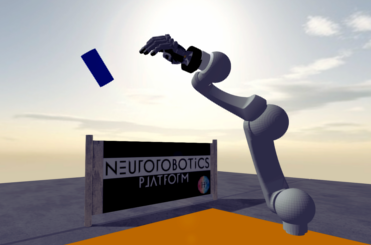
\includegraphics[width=0.4\textwidth]{hbpprak_2018}
	\end{center}
	\caption{The robot arm throwing the cylinder away from the table.}
	\label{fig:challenge}
\end{figure}

Sections \ref{sec:EA} and \ref{sec:MC} describe algorithms for solving optimization problems in general. Sections \ref{sec:firstApproach}, \ref{sec:secondApproach}, and \ref{sec:thirdApproach} describe our approaches for solving the Praktikum challenge.


\section{Evolutionary Algorithms} \label{sec:EA}

Evolutionary algorithms are population-based metaheuristics \cite{EA}. Metaheuristics are methods for solving optimization problems by iteratively improving candidate solutions in relation to a given quality measure.
Population-based metaheuristics use populations of multiple solutions and iteratively change populations to find a good solution.
An evolutionary algorithm is based on a population $P$ of possible solutions $e_i \in P$ for the optimization problem or heuristic to be solved. A solution is also referred to as an individual in the context of population-based metaheuristics.

In general, evolutionary algorithms consist of the following steps \cite{EA}:

\begin{enumerate}
\item Initialization: The initial population of individuals is generated randomly.

\item Evolutionary process: The individuals are evaluated by calculating their fitness. Therefore a fitness function is needed.
According to their fitness, some of the individuals are selected to be the parents of the following generation.
Then a process with reproduction, recombination, and mutation starts - similar to biological processes.
The parents are being recombinated and the resulting individuals are mutated to form the offspring of the current generation.
These steps are being repeated until a new population of individuals is generated. The parents are also added to the new population. This new population substitutes the old population and the process is repeated until an abort criterion is fulfilled  (see figure \ref{fig:EA}).

\item The best individual is selected.
\end{enumerate}


\begin{figure}
	\begin{center}
		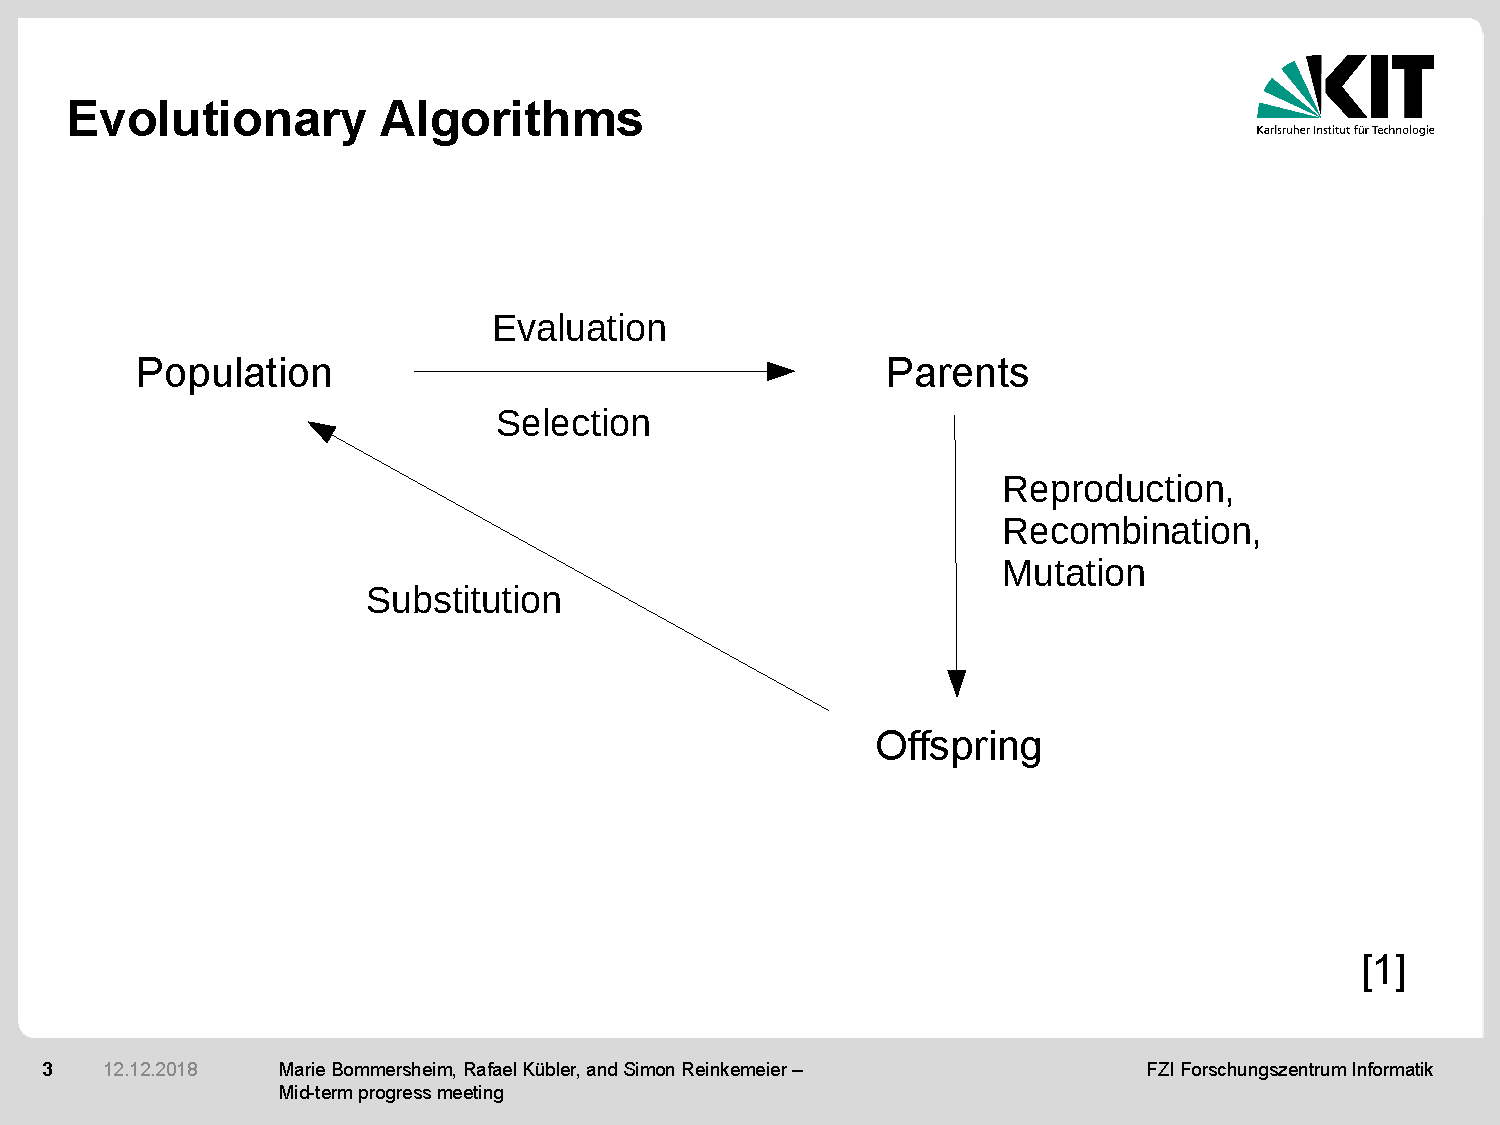
\includegraphics[trim = 2.2cm 6cm 4.2cm 6cm, clip, width=0.4\textwidth]{EA}
	\end{center}
	\caption{Evolutionary algorithms, adapted from \cite{EA}}
	\label{fig:EA}
\end{figure}

\section{Monte Carlo Algorithms} \label{sec:MC}

Monte Carlo algorithms are a class of computational algorithms \cite{MC}. They rely on repeated random sampling and provide generally aproximate solutions. Monte Carlo algorithms are used in cases where analytical or numerical solutions do not exist or are too difficult to implement.
In general, Monte Carlo algorithms consist of the following steps \cite{MC}:

\begin{enumerate}
\item Determine the statistical properties of possible inputs
\item Generate many sets of possible inputs which follows
the above properties
\item Perform a deterministic calculation with these sets
\item Analyze statistically the results
\end{enumerate}

Optimization problems are a possible application of Monte Carlo algorithms. Numerical solutions to optimization problems have the risk of getting stuck in local optima. The Monte Carlo approach can alleviate the problem by permitting random exit from the local optimum and find another, hopefully better optimum (see figure \ref{fig:MC}) \cite{MC}.

\begin{figure}
	\subfigure[A numerical solution found a local (not the global) minimum.]{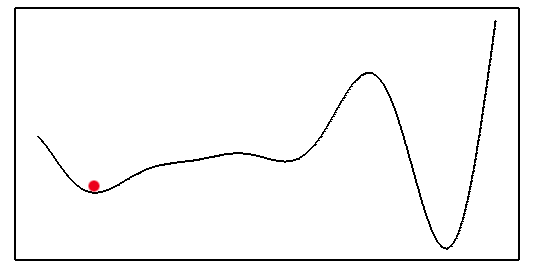
\includegraphics[width=0.23\textwidth]{MC1}}
	\hspace{1mm}
	\subfigure[Monte Carlo permits a random exit from local minimum.]{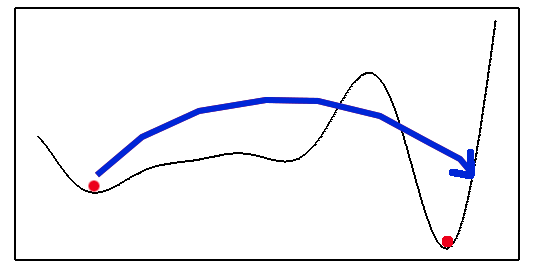
\includegraphics[width=0.23\textwidth]{MC2}}
	\caption{Monte Carlo algorithms are a possible method for solving optimization problems \cite{MC}.}
	\label{fig:MC}
\end{figure}

\section{First Approach} \label{sec:firstApproach}

The first approach is to let the robot arm hit the cylinder away from the table. Therefore, the movement is divided into three phases: reset, prepare, and hit. The phases are implemented as states using the state machine editor, the movements are hard-coded.

\begin{itemize}
\item Reset: Moves the arm in an upright position and puts the cylinder on the top right corner of the table (as seen from the robot arm).
\item Prepare: Moves the arm in an horizontal position pointing to 10 o'clock.
\item Hit: With a high acceleration, the arm moves towards the cylinder and knocks it off the table.
\end{itemize}

\section{Second Approach} \label{sec:secondApproach}

The second approach uses grasp and throw phases to throw the cylinder away from the table. The reset phase is taken from the first approach, the prepare phase from the first approach is adapted, the hit phase is replaced by the grasp and throw phases.
\begin{itemize}
\item Reset: Moves the arm in an upright position and puts the cylinder on the top right corner of the table (as seen from the robot arm).
\item Prepare: Moves the arm next to the cylinder (on the left as seen from the robot arm).
\item Grasp: Moves the fingers of the robot hand around the cylinder in order to hold it tight.
\item Throw: With high acceleration, the arm moves backwards beyond the vertical position and the hand opens to throw the cylinder away.
\end{itemize}

These movements are also hard-coded.

\section{Third Approach} \label{sec:thirdApproach}

This section describes two different ideas to optimize the throw movement. In both approaches the aim is to let the robot learn which movement is best to throw the cylinder as far away from the table as possible.

\subsection{Evolutionary Approach} \label{subsec:EA}

This approach uses the phases from the second approach. The reset, prepare, and grasp are still hard-coded as in the second approach. The throw phase is trained using an evolutionary algorithm. 

\subsection{Monte Carlo Approach} \label{subsec:MC}

This approach also uses the phases from the second approach. The reset, prepare, and grasp are still hard-coded as in the second approach. The throw phase is trained using a Monte Carlo algorithm. 

{\small
\bibliographystyle{ieee}
\bibliography{egbib}
}

\end{document}
